% Copyright 2015-2016 Jonathan Eyolfson
%
% This work is licensed under a Creative Commons Attribution-ShareAlike 4.0
% International License. You should have received a copy of the license along
% with this work. If not, see <http://creativecommons.org/licenses/by-sa/4.0/>.

\documentclass[10pt, draft]{book}

\usepackage{amsmath}
\usepackage{amssymb}
\usepackage{float}
\usepackage{fontspec}
\usepackage[a5paper, bindingoffset=10mm, inner=20mm, outer=20mm]{geometry}
\usepackage[newfloat]{minted}
\usepackage{tikz}

%% \setmainfont[Ligatures=TeX]{Tinos}
%% \setsansfont{Arimo}[Scale=MatchLowercase]
\setmonofont{Overpass Mono}[Scale=MatchLowercase]

\definecolor{solarizedBase03}{RGB}{0, 43, 54}
\definecolor{solarizedBase0}{RGB}{131, 148, 150}
\definecolor{solarizedBlue}{RGB}{38, 139, 210}

\usetikzlibrary{arrows, automata, decorations.pathreplacing, positioning}

\newcommand{\binary}[1]{$(\texttt{#1})_{2}$}
\newcommand{\hexadecimal}[1]{$(\texttt{#1})_{16}$}

\begin{document}

  \begin{titlepage}
    \begin{tikzpicture}[remember picture, overlay]
      \draw[draw=none, fill=solarizedBase03]
        (current page.north west) rectangle (current page.south east);
      \node[color=solarizedBlue, text width=1.75cm, text centered, scale=7]
        (title) at (current page.center) {\texttt{The Big Book of Computing}};
      \node[anchor=south west, inner sep=4mm, color=solarizedBase0, scale=1.5]
        at (current page.south west) {\texttt{0.0.1-development}};
      \node[anchor=south east, inner sep=4mm, color=solarizedBase0, scale=1.5]
        at (current page.south east) {\texttt{Jonathan Eyolfson}};
    \end{tikzpicture}
  \end{titlepage}

  \tableofcontents

  \newcommand{\helloworld}{``Hello, World!''}

\chapter{\helloworld{}}

The following page shows all you need for \helloworld{} using a Linux kernel on
an x86-64 processor.

\newpage

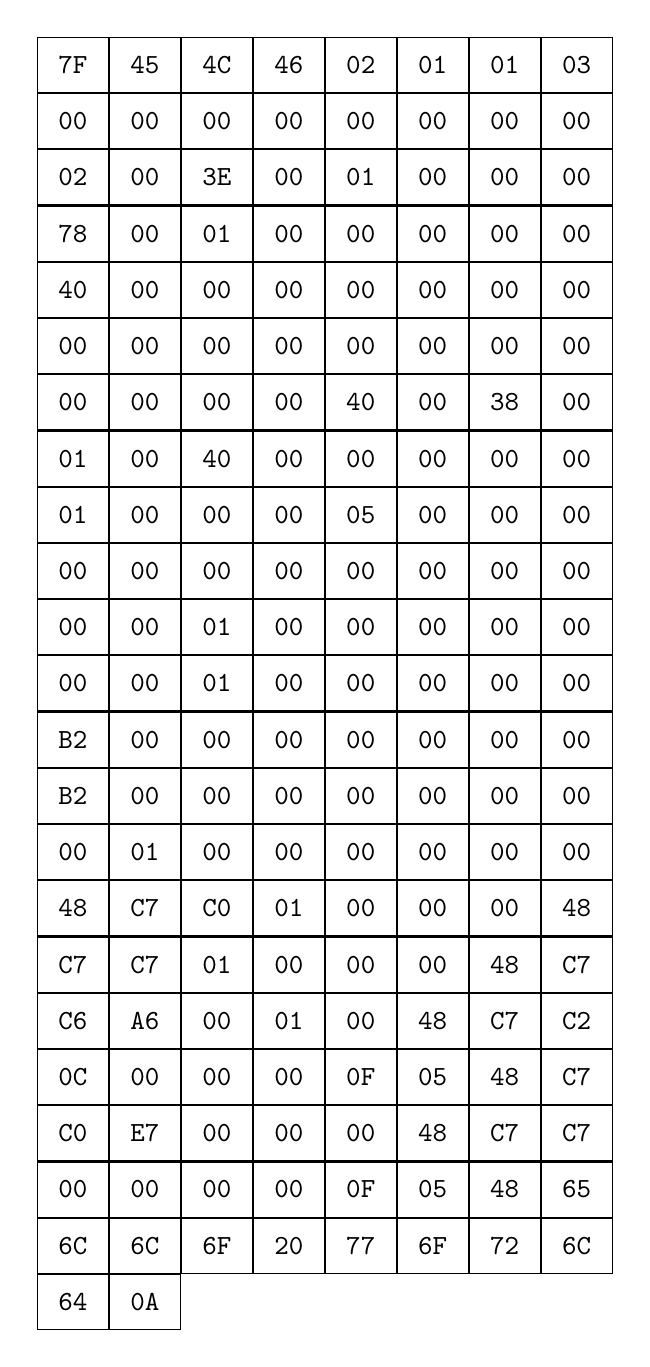
\begin{tikzpicture}[byte/.style={font=\ttfamily, draw, rectangle, minimum height=7mm, minimum width=9mm}]
  \matrix[column sep=0mm, row sep=0mm] {
    \node [byte] {7F}; &
    \node [byte] {45}; &
    \node [byte] {4C}; &
    \node [byte] {46}; &
    \node [byte] {02}; &
    \node [byte] {01}; &
    \node [byte] {01}; &
    \node [byte] {03}; \\

    \node [byte] {00}; &
    \node [byte] {00}; &
    \node [byte] {00}; &
    \node [byte] {00}; &
    \node [byte] {00}; &
    \node [byte] {00}; &
    \node [byte] {00}; &
    \node [byte] {00}; \\

    \node [byte] {02}; &
    \node [byte] {00}; &
    \node [byte] {3E}; &
    \node [byte] {00}; &
    \node [byte] {01}; &
    \node [byte] {00}; &
    \node [byte] {00}; &
    \node [byte] {00}; \\

    \node [byte] {78}; &
    \node [byte] {00}; &
    \node [byte] {01}; &
    \node [byte] {00}; &
    \node [byte] {00}; &
    \node [byte] {00}; &
    \node [byte] {00}; &
    \node [byte] {00}; \\

    \node [byte] {40}; &
    \node [byte] {00}; &
    \node [byte] {00}; &
    \node [byte] {00}; &
    \node [byte] {00}; &
    \node [byte] {00}; &
    \node [byte] {00}; &
    \node [byte] {00}; \\

    \node [byte] {00}; &
    \node [byte] {00}; &
    \node [byte] {00}; &
    \node [byte] {00}; &
    \node [byte] {00}; &
    \node [byte] {00}; &
    \node [byte] {00}; &
    \node [byte] {00}; \\

    \node [byte] {00}; &
    \node [byte] {00}; &
    \node [byte] {00}; &
    \node [byte] {00}; &
    \node [byte] {40}; &
    \node [byte] {00}; &
    \node [byte] {38}; &
    \node [byte] {00}; \\

    \node [byte] {01}; &
    \node [byte] {00}; &
    \node [byte] {40}; &
    \node [byte] {00}; &
    \node [byte] {00}; &
    \node [byte] {00}; &
    \node [byte] {00}; &
    \node [byte] {00}; \\

    \node [byte] {01}; &
    \node [byte] {00}; &
    \node [byte] {00}; &
    \node [byte] {00}; &
    \node [byte] {05}; &
    \node [byte] {00}; &
    \node [byte] {00}; &
    \node [byte] {00}; \\

    \node [byte] {00}; &
    \node [byte] {00}; &
    \node [byte] {00}; &
    \node [byte] {00}; &
    \node [byte] {00}; &
    \node [byte] {00}; &
    \node [byte] {00}; &
    \node [byte] {00}; \\

    \node [byte] {00}; &
    \node [byte] {00}; &
    \node [byte] {01}; &
    \node [byte] {00}; &
    \node [byte] {00}; &
    \node [byte] {00}; &
    \node [byte] {00}; &
    \node [byte] {00}; \\

    \node [byte] {00}; &
    \node [byte] {00}; &
    \node [byte] {01}; &
    \node [byte] {00}; &
    \node [byte] {00}; &
    \node [byte] {00}; &
    \node [byte] {00}; &
    \node [byte] {00}; \\

    \node [byte] {B2}; &
    \node [byte] {00}; &
    \node [byte] {00}; &
    \node [byte] {00}; &
    \node [byte] {00}; &
    \node [byte] {00}; &
    \node [byte] {00}; &
    \node [byte] {00}; \\

    \node [byte] {B2}; &
    \node [byte] {00}; &
    \node [byte] {00}; &
    \node [byte] {00}; &
    \node [byte] {00}; &
    \node [byte] {00}; &
    \node [byte] {00}; &
    \node [byte] {00}; \\

    \node [byte] {00}; &
    \node [byte] {01}; &
    \node [byte] {00}; &
    \node [byte] {00}; &
    \node [byte] {00}; &
    \node [byte] {00}; &
    \node [byte] {00}; &
    \node [byte] {00}; \\

    \node [byte] {48}; &
    \node [byte] {C7}; &
    \node [byte] {C0}; &
    \node [byte] {01}; &
    \node [byte] {00}; &
    \node [byte] {00}; &
    \node [byte] {00}; &
    \node [byte] {48}; \\

    \node [byte] {C7}; &
    \node [byte] {C7}; &
    \node [byte] {01}; &
    \node [byte] {00}; &
    \node [byte] {00}; &
    \node [byte] {00}; &
    \node [byte] {48}; &
    \node [byte] {C7}; \\

    \node [byte] {C6}; &
    \node [byte] {A6}; &
    \node [byte] {00}; &
    \node [byte] {01}; &
    \node [byte] {00}; &
    \node [byte] {48}; &
    \node [byte] {C7}; &
    \node [byte] {C2}; \\

    \node [byte] {0C}; &
    \node [byte] {00}; &
    \node [byte] {00}; &
    \node [byte] {00}; &
    \node [byte] {0F}; &
    \node [byte] {05}; &
    \node [byte] {48}; &
    \node [byte] {C7}; \\

    \node [byte] {C0}; &
    \node [byte] {E7}; &
    \node [byte] {00}; &
    \node [byte] {00}; &
    \node [byte] {00}; &
    \node [byte] {48}; &
    \node [byte] {C7}; &
    \node [byte] {C7}; \\

    \node [byte] {00}; &
    \node [byte] {00}; &
    \node [byte] {00}; &
    \node [byte] {00}; &
    \node [byte] {0F}; &
    \node [byte] {05}; &
    \node [byte] {48}; &
    \node [byte] {65}; \\

    \node [byte] {6C}; &
    \node [byte] {6C}; &
    \node [byte] {6F}; &
    \node [byte] {20}; &
    \node [byte] {77}; &
    \node [byte] {6F}; &
    \node [byte] {72}; &
    \node [byte] {6C}; \\

    \node [byte] {64}; &
    \node [byte] {0A}; \\
  };
\end{tikzpicture}

  \chapter{Mathematical Basics}

Understand the following terminology: commutativity, and associativity.

\section{Numeral Systems}

\subsection{Decimal}

The number system you're use to is base 10. A number such as 101 can be broken
down by looking at the value associated with every digit. The numeral system
we're all familiar with is base 10. We start by associating the last digit with
the value 1 ($10^0$) and increase this value by a factor of 10 for each digit
as we work from right to left. We can break down 101 in the following chart:

\begin{center}
  \begin{tabular}{r | r | r}
    $10^2$ & $10^1$ & $10^0$ \\
    \hline
         1 &      0 &      1 \\
  \end{tabular}
\end{center}

\label{sec:numeral-system-binary}
\subsection{Binary}

\begin{center}
  \begin{tabular}{r | r | r}
    $2^2$ & $2^1$ & $2^0$ \\
    \hline
        1 &      0 &      1 \\
  \end{tabular}

  \vspace{1em}

  $= 2^2 \times 1 + 2^1 \times 0 + 2^0 \times 1 = 4 \times 1 + 1 \times 1 = 5
   = (101)_2$
\end{center}

\subsection{Octal}

This is the same as before, except now it's base 8.

\subsection{Hexadecimal}

Same as binary and octal, except instead of base 2 you use base 16.

\begin{tabular}{c c}
  \hline
  Value & Equivalent \\
  \hline
  10 & $(\text{A})_{16}$ \\
  11 & $(\text{B})_{16}$ \\
  12 & $(\text{C})_{16}$ \\
  13 & $(\text{D})_{16}$ \\
  14 & $(\text{E})_{16}$ \\
  15 & $(\text{F})_{16}$ \\
\end{tabular}

For instance: $95 = (5\text{F})_{16}$.

  \chapter{Booleans}

\section{Algebra}

\subsection{Basics}

There are 3 basic operations: \textbf{and}, \textbf{or}, and \textbf{not}. These
3 operations may go by their fancier names: \textbf{conjunction},
\textbf{disjunction}, and \textbf{negation}. The mathematical shorthand for
these 3 operations are: $\land$, $\lor$, and $\lnot$.

The first 2 operations take two booleans and produce another boolean value
(similar to addition for numbers). Since the value of a boolean can only be 0 or
1, we can enumerate all the different possibilities for these operations.  This
is shown in a truth table below:

\begin{center}
  \begin{tabular}{r r | r | r}
    $x$ & $y$ & $\land$ & $\lor$ \\
    \hline
    0 &   0 &       0 &      0 \\
    0 &   1 &       0 &      1 \\
    1 &   0 &       0 &      1 \\
    1 &   1 &       1 &      1 \\
  \end{tabular}
\end{center}

The last operation, \textbf{not}, takes one boolean value and changes its
value. So, $\lnot 0 = 1$ and $\lnot 1 = 0$.

\subsection{Derived}

There are 3 dervied operations: \textbf{equivalence}, \textbf{exclusive or
(xor)}, and \textbf{material implication}. The mathematical shorthand for these
3 operations are: $\equiv$, $\oplus$, and $\to$. Their truth table is shown
below:

\begin{center}
  \begin{tabular}{r r | r | r | r}
    $x$ & $y$ & $\equiv$ & $\oplus$ & $\to$ \\
    \hline
    0 &   0 &        1 &        0 &     1 \\
    0 &   1 &        0 &        1 &     0 \\
    1 &   0 &        0 &        1 &     1 \\
    1 &   1 &        1 &        0 &     1 \\
  \end{tabular}
\end{center}

  \chapter{Encodings}

First rule: everything in computing is a number. Everything boils down to a
sequence of booleans. When talking about booleans stored on a computer we use
the synonym bit instead. A bit is short for binary digit, which is either 0 or
1. The smallest unit stored on a computer is typically 8 bits (8 b), this unit
is called a byte (1 B).

\section{Numbers}

Unlike in pure mathematics where we can write numbers up to infinity we are
constrained by bytes on a computer. Doing strict math can easily result in
errors and wrong results. We need to be able to understand these issues so we do
not produce incorrect answers.

\begin{quote}
  “An ounce of prevention is worth a pound of cure.”

  --- Benjamin Franklin
\end{quote}

\subsection{Naturals}

The values here are exactly like the binary numeral system in
\textbf{Section~\ref{sec:numeral-system-binary}}.

\subsection{Integers}

The most popular integer encoding is \textbf{two's complement}. The sign is
encoded in the \textbf{most significant bit (MSB)}. A value of 0 indicates the
number is positive and the value is the same as the natural number value of the
remaining bits. A value of 1 indicates the number is negative and the value is
obtained from negating all the bits, adding one, and taking the value as the
natural number value of all the bits.

\newpage
\section{Character}

\subsection{ASCII}

{\scriptsize\ttfamily\begin{tabular}{c c}
  \hline
  Value & Meaning \\
  \hline
    0 & \colorbox{gray}{NUL} \\
    1 & \colorbox{gray}{SOH} \\
    2 & \colorbox{gray}{STX} \\
    3 & \colorbox{gray}{ETX} \\
    4 & \colorbox{gray}{EOT} \\
    5 & \colorbox{gray}{ENQ} \\
    6 & \colorbox{gray}{ACK} \\
    7 & \colorbox{gray}{BEL} \\
    8 & \colorbox{gray}{BS} \\
    9 & \colorbox{gray}{HT} \\
   10 & \colorbox{gray}{LF} \\
   11 & \colorbox{gray}{VT} \\
   12 & \colorbox{gray}{FF} \\
   13 & \colorbox{gray}{CR} \\
   14 & \colorbox{gray}{SO} \\
   15 & \colorbox{gray}{SI} \\
   16 & \colorbox{gray}{DLE} \\
   17 & \colorbox{gray}{DC1} \\
   18 & \colorbox{gray}{DC2} \\
   19 & \colorbox{gray}{DC3} \\
   20 & \colorbox{gray}{DC4} \\
   21 & \colorbox{gray}{NAK} \\
   22 & \colorbox{gray}{SYN} \\
   23 & \colorbox{gray}{ETB} \\
   24 & \colorbox{gray}{CAN} \\
   25 & \colorbox{gray}{EM} \\
   26 & \colorbox{gray}{SUB} \\
   27 & \colorbox{gray}{ESC} \\
   28 & \colorbox{gray}{FS} \\
   29 & \colorbox{gray}{GS} \\
   30 & \colorbox{gray}{RS} \\
   31 & \colorbox{gray}{US} \\
\end{tabular}
\quad
\begin{tabular}{c c}
  \hline
  Value & Meaning \\
  \hline
   32 & \colorbox{gray}{SPACE} \\
   33 & ! \\
   34 & " \\
   35 & \# \\
   36 & \$ \\
   37 & \% \\
   38 & \& \\
   39 & ' \\
   40 & ( \\
   41 & ) \\
   42 & * \\
   43 & + \\
   44 & , \\
   45 & - \\
   46 & . \\
   47 & / \\
   48 & 0 \\
   49 & 1 \\
   50 & 2 \\
   51 & 3 \\
   52 & 4 \\
   53 & 5 \\
   54 & 6 \\
   55 & 7 \\
   56 & 8 \\
   57 & 9 \\
   58 & : \\
   59 & ; \\
   60 & < \\
   61 & = \\
   62 & > \\
   63 & ? \\
\end{tabular}
\quad
\begin{tabular}{c c}
  \hline
  Value & Meaning \\
  \hline
   64 & @ \\
   65 & A \\
   66 & B \\
   67 & C \\
   68 & D \\
   69 & E \\
   70 & F \\
   71 & G \\
   72 & H \\
   73 & I \\
   74 & J \\
   75 & K \\
   76 & L \\
   77 & M \\
   78 & N \\
   79 & O \\
   80 & P \\
   81 & Q \\
   82 & R \\
   83 & S \\
   84 & T \\
   85 & U \\
   86 & V \\
   87 & W \\
   88 & X \\
   89 & Y \\
   90 & Z \\
   91 & [ \\
   92 & \textbackslash \\
   93 & ] \\
   94 & \textasciicircum \\
   95 & \_ \\
\end{tabular}
\quad
\begin{tabular}{c c}
  \hline
  Value & Meaning \\
  \hline
   96 & ` \\
   97 & a \\
   98 & b \\
   99 & c \\
  100 & d \\
  101 & e \\
  102 & f \\
  103 & g \\
  104 & h \\
  105 & i \\
  106 & j \\
  107 & k \\
  108 & l \\
  109 & m \\
  110 & n \\
  111 & o \\
  112 & p \\
  113 & q \\
  114 & r \\
  115 & s \\
  116 & t \\
  117 & u \\
  118 & v \\
  119 & w \\
  120 & x \\
  121 & y \\
  122 & z \\
  123 & \{ \\
  124 & | \\
  125 & \} \\
  126 & \textasciitilde \\
  127 & \colorbox{gray}{DEL} \\
\end{tabular}}

\newpage
\section{Data}

\subsection{Base64}

The following is a table of the encoded values:

{\ttfamily\begin{tabular}{c c}
  \hline
  Value & ASCII Character \\
  \hline
   0 & A \\
   1 & B \\
   2 & C \\
   3 & D \\
   4 & E \\
   5 & F \\
   6 & G \\
   7 & H \\
   8 & I \\
   9 & J \\
  10 & K \\
  11 & L \\
  12 & M \\
  13 & N \\
  14 & O \\
  15 & P \\
  16 & Q \\
  17 & R \\
  18 & S \\
  19 & T \\
  20 & U \\
  21 & V \\
  22 & W \\
  23 & X \\
  24 & Y \\
  25 & Z \\
  26 & a \\
  27 & b \\
  28 & c \\
  29 & d \\
  30 & e \\
  31 & f \\
\end{tabular}
\quad
\begin{tabular}{c c}
  \hline
  Value & ASCII Character \\
  \hline
  32 & g \\
  33 & h \\
  34 & i \\
  35 & j \\
  36 & k \\
  37 & l \\
  38 & m \\
  39 & n \\
  40 & o \\
  41 & p \\
  42 & q \\
  43 & r \\
  44 & s \\
  45 & t \\
  46 & u \\
  47 & v \\
  48 & w \\
  49 & x \\
  50 & y \\
  51 & z \\
  52 & 0 \\
  53 & 1 \\
  54 & 2 \\
  55 & 3 \\
  56 & 4 \\
  57 & 5 \\
  58 & 6 \\
  59 & 7 \\
  60 & 8 \\
  61 & 9 \\
  62 & + \\
  63 & / \\
\end{tabular}}

Each encoded value represents 6 bits. Each group is 4 characters long.
Therefore these 4 characters represent 3 bytes (`=' is used for padding).

  \chapter{Arithmetic}

Assuming a background with the following functions:

\begin{equation*}
  \text{floor}(x) = \lfloor x \rfloor = \max\{m \in \mathbb{Z} \mid m \leq x \}
\end{equation*}

\begin{equation*}
  \text{ceiling}(x) = \lceil x \rceil = \min\{n \in \mathbb{Z} \mid n \geq x \}
\end{equation*}

\begin{equation*}
\mathrm{trunc}(x) = \begin{cases}
\lfloor x \rfloor &\text{if $x \geq 0$,}\\
\lceil x \rceil &\text{otherwise.}
\end{cases}
\end{equation*}

\section{Division}

Every computer scientist and engineer needs to know the details of natural
number and integer division \cite{division-and-modulus-for-computer-scientists}.

Dividend / Divisor = (Quotient, Remainder)

$a / b = (q, r)$

where

$a = bq + r$

If you just want the remainder, the operation is $a \bmod b$.

there's a unique answer for $a, b$ when $0 \leq r < |b|$.

\begin{align*}
a &= 7  & b &= 3  & q &= 2  & r &= 1\\
a &= 7  & b &= -3 & q &= -2 & r &= 1\\
a &= -7 & b &= 3  & q &= -3 & r &= 2\\
a &= -7 & b &= -3 & q &= 3  & r &= 2
\end{align*}

But, in \texttt{python} (using \texttt{//} for floor divison):

\begin{align*}
a &= 7  & b &= 3  & q &= 2  & r &= 1\\
a &= 7  & b &= -3 & q &= -3 & r &= -2\\
a &= -7 & b &= 3  & q &= -3 & r &= 2\\
a &= -7 & b &= -3 & q &= 2  & r &= -1
\end{align*}

However, if we use truncated divison (\texttt{C/C++}):

\begin{align*}
a &= 7  & b &= 3  & q &= 2  & r &= 1\\
a &= 7  & b &= -3 & q &= -2 & r &= 1\\
a &= -7 & b &= 3  & q &= -2 & r &= -1\\
a &= -7 & b &= -3 & q &= 2  & r &= -1
\end{align*}

\subsection{Truncated}

In truncated division:

$q = \textrm{trunc}(\frac{a}{b})$

$r = a - b\ \textrm{trunc}(\frac{a}{b})$

Same sign as the dividend (it should say unless it's zero!).

Case 1)
If $a$ is negative.

Case 1a)
If $b$ is positive then $r = a - b \lceil \frac{a}{b} \rceil$.
Then $a \leq b \lceil \frac{a}{b} \rceil$ because it rounds up (division is
negative).
\textbf{OR.}
Divide both sides by $b$ giving $\frac{a}{b} \leq \lceil \frac{a}{b} \rceil$,
which is clearly true.

Case 1b)
If $b$ is negative then $r = a - b \lfloor \frac{a}{b} \rfloor$.
Then $a \leq b \lfloor \frac{a}{b} \rfloor$ because it rounds down (division is
positive).
So it's a negative multiplied by a smaller positive number than without the
floor, resulting in a larger result.
\textbf{OR.}
Divide both sides by $b$ ($b$ is negative so flip the inequality) giving
$\frac{a}{b} \geq \lfloor \frac{a}{b} \rfloor$, which is clearly true.

Case 2)
If $a$ is positive.

Case 2a)
If $b$ is positive then $r = a - b \lfloor \frac{a}{b} \rfloor$.
We know $a \geq b \lfloor \frac{a}{b} \rfloor$.
So $r$ is positive.

Case 2b)
If $b$ is negative then $r = a - b \lceil \frac{a}{b} \rceil$.
To be postive then $a \geq b \lceil \frac{a}{b} \rceil$.
Divide both sides by $b$ giving $a \leq \lceil \frac{a}{b} \rceil$.
So $r$ is positive.

\subsection{Floored}

In floored division:

$q = \lfloor \frac{a}{b} \rfloor$

$r = a - b \lfloor \frac{a}{b} \rfloor$

If $b$ is positive.

$\frac{a}{b} \geq \lfloor \frac{a}{b} \rfloor$

Result is positive.

If $b$ is negative.

$\frac{a}{b} \leq \lfloor \frac{a}{b} \rfloor$

Result is negative.

\subsection{Euclidean}

\subsection{Example}

\begin{lstlisting}
uint8_t mean(uint8_t x_0, uint8_t x_1)
{
  return (x_0 + x_1) / 2;
}
\end{lstlisting}

Wrong! Poor understanding of both \texttt{+} and \texttt{/}.

If $x_0 = 201$ and $x_1 = 203$, then $\text{mean}(x_0, x_1) = 202$.

Since all numbers are positive, it doesn't matter which div or mod functions we
use.
This code is the following:

\begin{equation*}
  \text{div}(\text{mod}(x_0 + x_1, 2^{8}), 2)
\end{equation*}

\begin{lstlisting}
uint8_t mean(uint8_t x_0, uint8_t x_1)
{
  return (x_0 / 2) + (x_1 / 2);
}
\end{lstlisting}

Also wrong. Probably even worse, it gives the wrong result whenever both numbers
are odd. The mod function will never not equal $a$ (or no overflow).

\begin{equation*}
  \text{div}(x_0 , 2) + \text{div}(x_1 , 2) \neq \text{div}(x_0 + x_1, 2)
\end{equation*}

\begin{equation*}
  \lfloor \frac{x_0}{2} \rfloor + \lfloor \frac{x_1}{2} \rfloor
  \neq \lfloor \frac{x_0 + x_1}{2} \rfloor
\end{equation*}

\begin{equation*}
  \lfloor \frac{x_0}{2} \rfloor + \lfloor \frac{x_1}{2} \rfloor
  + \lfloor \frac{\text{mod}(x_0, 2) + \text{mod}(x_1, 2)}{2} \rfloor
  = \lfloor \frac{x_0 + x_1}{2} \rfloor
\end{equation*}

  \chapter{Algorithms}

\section{Sorting}

\section{Searching}

\section{Scheduling}

\section{Hill Climbing}

  \chapter{Nintendo Entertainment System}

It's CPU is a \textit{MOS Technology 6502}.
The is an 8-bit microprocessor.

  \chapter{Hardware}

  \chapter{Teensy 3.2}

\section{Hardware}

System on chip (SoC) is MK20DX256VLH7.

\begin{description}
  \item[CPU.] ARM Cortex M4
  \item[Storage.] 256 K Flash
  \item[RAM.] 64 K
  \item[ROM.] 2 K EEPROM
\end{description}

Components:

\begin{description}
  \item[LP38691.] (1) 500 mA Low Dropout CMOS Linear Regulators Stable with
                  Ceramic Output Capacitors
  \item[MKL02Z32VFG4.] (1) ARM Cortex-M0+ Kinetis KL02 Microcontroller IC 32-Bit
                       48MHz 32KB (32K x 8) FLASH 16-QFN (3x3)
  \item[MK20DX256VLH7.] ARM Cortex-M4 Kinetis K20 Microcontroller IC 32-Bit
                        72MHz 256KB (256K x 8) FLASH 64-LQFP
                        (10x10)
\end{description}

The is a secondary CPU containing the \textit{HalfKay bootloader}.
A special USB packet or pressing the on-board button activates this CPU.
It uploads the bootloader code to the main RAM and tells the main CPU to
execute it(?).
The bootloader clears flash and writes the flash with new code, afterwards it
reboots itself.

PTA18 and PTA19 are connected to a 16 MHz clock.

CPU is at 48 MHz or 48,000,000 times a second.

\texttt{SYST\_RVR} is 47,999 or \hexadecimal{BB7F}.
Since it counts down to 0, the SysTick interrupt occurs at 1,000 kHz.
In other words it occurs every ms (millisecond).

\texttt{SYST\_CSR} is \hexadecimal{7}.
Core clock is used for systick.
Generates a SysTick interrupt when 0.
Counter operates in multi-shot manner.

\newpage
\section{Blinking LED}

The hex file to transfer to the Teensy is actually 14324 bytes.
Let's see if we can account for all 14324 bytes.
All instructions are at least 2 bytes, giving a maximum of 7162 instructions.

The address \hexadecimal{00 00 00 00} is the vector table. This table contains
addresses for each entry. Only entry 0, 1, and 15 are important for now.

Minimum alignment is 128 bytes (32 addresses). The first entry is the stack
pointer, all others are destinations of a branch and must have bit 0 set to 1.

[\hexadecimal{00 00 31 F0}, \hexadecimal{00 00 37 F4}) are part of the data
section. This accounts for 1540 bytes. It's copied to
[\hexadecimal{1F FF 84 40}, \hexadecimal{1F FF 8A 44}).

The zero'ed memory section does not take up any space in the executable itself
but does exist in RAM. The zero'ed section is the addresses in the range
[\hexadecimal{1F FF 8A 44}, \hexadecimal{1F FF 8E 2C}).
This takes up 1000 bytes.

\subsection{Execution}

The following is the program flow:

\indent \texttt{ResetHandler (mk20dx128.c)}

\hspace{2mm} \texttt{startup\_early\_hook (mk20dx128.c)}

\hspace{2mm} \texttt{\_init\_Teensyduino\_internal\_ (pins\_teensy.c)}

\hspace{4mm} \texttt{analog\_init (analog.c)}

\hspace{4mm} \texttt{delay(4) (pins\_teensy.c)}

\hspace{4mm} \texttt{usb\_init (usb\_dev.c)}

\hspace{6mm} \texttt{usb\_init\_serialnumber (usb\_desc.c)}

\hspace{8mm} \texttt{ultoa (nonstd.c)}

\subsection{Functions}

\paragraph{\texttt{ResetHandler (mk20dx128.c)}} Reset interrupt handler.

\hexadecimal{00 00 01 BC} is load watchdog address.

\vspace{1em}

\hexadecimal{00 00 02 0C} is data copy loop setup start.

\hexadecimal{00 00 02 14} is the initial branch into the conditional check.

\hexadecimal{00 00 02 16} is the start of the loop body.

\hexadecimal{00 00 02 1A} is the end of the loop body.

\hexadecimal{00 00 02 1C} is the start of the conditional check.

\hexadecimal{00 00 02 20} conditional branch back into loop.

\vspace{1em}

\hexadecimal{00 00 02 22} is data copy loop setup start.

\hexadecimal{00 00 02 30} conditional branch back into loop.

\vspace{1em}

\hexadecimal{00 00 02 44} conditional branch back into loop (int. priority).

\vspace{1em}

\hexadecimal{00 00 02 D8} is \texttt{\_\_enable\_irq}.

\hexadecimal{00 00 02 DA} call to \texttt{\_init\_Teensyduino\_internal\_}

\vspace{1em}

\hexadecimal{00 00 03 40} is \texttt{MCG\_S} address (4 bytes).

\hexadecimal{00 00 03 44} is \texttt{MCG\_C5} address (4 bytes).

\hexadecimal{00 00 03 54} is \texttt{SIM\_CLKDIV2} address (4 bytes).

\hexadecimal{00 00 03 58} is \texttt{SIM\_SOPT2} constant value (4 bytes).

\hexadecimal{00 00 03 5C} is \texttt{SYST\_RVR} address (4 bytes).

\paragraph{\texttt{??? (???)}} Enables Port A-E IRQs.

\hexadecimal{00 00 05 08} is entry point.

\hexadecimal{00 00 05 28} is exit point.

\hexadecimal{00 00 05 2A} is empty padding (2 bytes) [?].

\hexadecimal{00 00 05 2C} is \texttt{NVIC\_ISER2} address (4 bytes).

\textbf{Total: 40 bytes}


\paragraph{\texttt{micros (pins\_teensy.c)}} Returns current time in
microseconds.

\hexadecimal{00 00 08 10} is \texttt{\_\_disable\_irq}.

\hexadecimal{00 00 08 1E} is \texttt{\_\_enable\_irq}.

\hexadecimal{00 00 08 3E} is \texttt{return ...}.

\vspace{1em}

\hexadecimal{00 00 08 40} is \texttt{SYST\_CVR} address (4 bytes).

\hexadecimal{00 00 08 44} is \texttt{ICSR} address (4 bytes).

\hexadecimal{00 00 08 48} is \texttt{systick\_millis\_count} address (4 bytes).

\textbf{Total: 60 bytes}

\paragraph{\texttt{delay (pins\_teensy.c)}} Delays the processor at least
specified number of milliseconds.

\hexadecimal{00 00 08 4C} is entry point (push \texttt{R4}, \texttt{R5},
\texttt{R6}, \texttt{R14}).

\hexadecimal{00 00 08 50} is call to \texttt{micros()} for \texttt{start}.

\hexadecimal{00 00 08 5C} is call to \texttt{micros()} in \texttt{while}.

\hexadecimal{00 00 08 6E} is \texttt{yield()}.

\hexadecimal{00 00 08 68} is conditional branch to \texttt{return}.

\hexadecimal{00 00 08 74} is \texttt{return} (with \texttt{POP}).

\hexadecimal{00 00 08 76} is empty padding (2 bytes) [?].

\textbf{Total: 44 bytes}

\paragraph{\texttt{\_init\_Teensyduino\_internal\_ (pins\_teensy.c)}}
Init.

\hexadecimal{00 00 08 78} is entry (push \texttt{R4}, \texttt{R14}).

\hexadecimal{00 00 08 7A} is branch to enable port A-E IRQs.

\hexadecimal{00 00 08 CA} call to \texttt{delay} (4 bytes)

\hexadecimal{00 00 08 CE} return from \texttt{delay} (4 bytes) (pop \texttt{R4},
\texttt{R5}, \texttt{R6}, \texttt{R14}).

\hexadecimal{00 00 08 D2} is branch to \texttt{usb\_init}.

\vspace{1em}

\hexadecimal{00 00 08 D8} is \texttt{FTM0\_CNT} address (4 bytes).

\hexadecimal{00 00 08 DC} is \texttt{FTM0\_C0SC} address (4 bytes).

\hexadecimal{00 00 08 E0} is \texttt{FTM0\_SC} address (4 bytes).

\hexadecimal{00 00 08 E4} is \texttt{FTM1\_CNT} address (4 bytes).

\hexadecimal{00 00 08 E8} is \texttt{FTM2\_CNT} address (4 bytes).

\hexadecimal{00 00 08 EC} is \texttt{FTM2\_MOD} address (4 bytes).

\hexadecimal{00 00 08 F0} is \texttt{FTM2\_C0SC} address (4 bytes).

\hexadecimal{00 00 08 F4} is \texttt{FTM2\_SC} address (4 bytes).

\textbf{Total: 128 bytes}

\paragraph{\texttt{yield (???)}} Unknown.

\hexadecimal{00 00 10 00} is an immediate return.

\textbf{Total: 2 bytes}

\paragraph{\texttt{startup\_early\_hook (mk20dx128.c)}} Default, allows updates
to the watchdog.

\hexadecimal{00 00 13 88} is entry point.

\hexadecimal{00 00 13 8E} is \texttt{return}.

\hexadecimal{00 00 13 90} is \texttt{WDOG\_STCTRLH} address.

\textbf{Total: 12 bytes}

\paragraph{\texttt{usb\_init\_serialnumber (usb\_desc.c)}} Set serial number.

\hexadecimal{00 00 13 E4} is entry point.
(push \texttt{R0}, \texttt{R1}, \texttt{R2}, \texttt{R3},
\texttt{R4}, \texttt{R14})

\hexadecimal{00 00 14 0E} is branch to \texttt{ultoa}.

\hexadecimal{00 00 14 12} is return from \texttt{ultoa}.

\hexadecimal{00 00 14 30} is move stack pointer up 5 values.

\hexadecimal{00 00 14 32} is return (pop \texttt{R15}).

\vspace{1em}

\hexadecimal{00 00 14 34} is \texttt{FTFL\_FSTAT} address (4 bytes).

\hexadecimal{00 00 14 38} is \texttt{FTFL\_FCCOB0} address (4 bytes).

\hexadecimal{00 00 14 3C} is \texttt{FTFL\_FCCOB7} address (4 bytes).

\hexadecimal{00 00 14 40} is {\tiny
\texttt{usb\_string\_serial\_number\_default}} address (4 bytes).

\textbf{Total: 96 bytes}

\paragraph{\texttt{usb\_init (usb\_dev.c)}} Unknown

\hexadecimal{00 00 1C 0C} is entry point (push \texttt{R3} and \texttt{R14}).

\hexadecimal{00 00 1C 0E} is branch to \texttt{usb\_init\_serialnumber}.

\hexadecimal{00 00 1C 12} is return from \texttt{usb\_init\_serialnumber}.

\paragraph{\texttt{ultoa (nonstd.c)}} Convert integer to string (with radix).

\hexadecimal{00 00 1D 28} is entry point (push \texttt{R4} and \texttt{R14}).

\hexadecimal{00 00 1D 62} is exit (pop \texttt{R4} and \texttt{R15}) (2 bytes).

\textbf{Total: 60 bytes}

\paragraph{\texttt{analog\_init (analog.c)}} Unknown

\hexadecimal{00 00 20 9C} is entry point.

\hexadecimal{00 00 21 26} is exit point.

\hexadecimal{00 00 21 28} is \texttt{VREF\_TRM} address (4 bytes).

\hexadecimal{00 00 21 2C} is \texttt{analog\_config\_bits} address (4 bytes).

\hexadecimal{00 00 21 30} is \texttt{ADC0\_CFG1} address (4 bytes).

\hexadecimal{00 00 21 34} is \texttt{ADC0\_CFG2} address (4 bytes).

\hexadecimal{00 00 21 38} is \texttt{ADC1\_CFG1} address (4 bytes).

\hexadecimal{00 00 21 40} is \texttt{analog\_reference\_internal} address
(4 bytes).

\hexadecimal{00 00 21 44} is \texttt{ADC0\_SC2} address (4 bytes).

\hexadecimal{00 00 21 48} is \texttt{ADC1\_SC2} address (4 bytes).

\hexadecimal{00 00 21 4C} is \texttt{analog\_num\_average} address (4 bytes).

\hexadecimal{00 00 21 50} is \texttt{ADC0\_SC3} address (4 bytes).

\hexadecimal{00 00 21 54} is \texttt{ADC1\_SC3} address (4 bytes).

\hexadecimal{00 00 21 58} is \texttt{calibrating} address (4 bytes).

\textbf{Total: 192 bytes}

\subsection{Variables}

Below are all the variables:

\vspace{1em}

\hexadecimal{1F FF 85 22} is {\tiny
\texttt{usb\_string\_serial\_number\_default}} struct (12 bytes).

\hexadecimal{1F FF 85 3C} is \texttt{analog\_config\_bits} value (1 byte).

\hexadecimal{1F FF 85 3D} is \texttt{analog\_num\_average} (1 byte).

\hexadecimal{1F FF 8A E8} is \texttt{systick\_millis\_count} (4 bytes).

\hexadecimal{1F FF 8D 6A} is \texttt{calibrating} (1 byte).

\hexadecimal{1F FF 8D 6B} is \texttt{analog\_reference\_internal} (1 byte).

\hexadecimal{?? ?? ?? ??} is \texttt{analog\_right\_shift} (1 byte).


  \chapter{Instruction Set Architecture}

Processors understand bytes in groups of different sizes. The representation of
this grouping is different on various processors. When we're using this data, we
understand it fully as a group and don't break it up into different parts. We
consider these groups to be \textbf{words} (their term not mine). We would
naturally understand a group of bytes with the most significant byte written to
the left writing the next least significant byte to the right. For instance, a 4
byte word is shown below with the least significant byte being 0-indexed.

\begin{center}
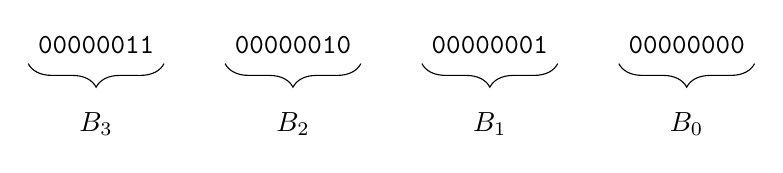
\begin{tikzpicture}
  \node (b3) {\ttfamily 00000011};
  \draw[decorate,decoration={amplitude=3mm,brace,mirror}]
    (b3.south west) -- (b3.south east);
  \node[below of=b3,anchor=center]{$B_3$};

  \node[right of=b3,node distance=2.5cm] (b2) {\ttfamily 00000010};
  \draw[decorate,decoration={amplitude=3mm,brace,mirror}]
    (b2.south west) -- (b2.south east);
  \node[below of=b2,anchor=center]{$B_2$};

  \node[right of=b2,node distance=2.5cm] (b1) {\ttfamily 00000001};
  \draw[decorate,decoration={amplitude=3mm,brace,mirror}]
    (b1.south west) -- (b1.south east);
  \node[below of=b1,anchor=center]{$B_1$};

  \node[right of=b1,node distance=2.5cm] (b0) {\ttfamily 00000000};
  \draw[decorate,decoration={amplitude=3mm,brace,mirror}]
    (b0.south west) -- (b0.south east);
  \node[below of=b0,anchor=center]{$B_0$};
\end{tikzpicture}
\end{center}

\section{ARM}

Currently, the plan is to initially make this secton specifically for ARMv7.

\section{x86-64}

\begin{listing}[H]
  \inputminted[frame=lines]{asm}{code/hello_world.asm}
  \caption{``Hello world'' program written in x86-64 assembly for Linux}
  \label{lst:hello-world-asm}
\end{listing}

Assuming the file is called ``\mintinline{console}{hello_world.asm}'' we need to
compile to machine code using \mintinline{console}{nasm -f elf64
  hello_world.asm}. This produces a file named
``\mintinline{console}{hello_world.o}'' which is an object file (more later). To
produce an executable file that will run on the machine use the standard linker:
\mintinline{console}{ld hello_world.o -o hello_world}. This produces an
executable named ``\mintinline{console}{hello_world}''. Running the program
using \mintinline{console}{./hello_world} produces the output
``\mintinline{console}{Hello world!}''.

x86-64 has 16 general purpose registers: \mintinline{asm}{rax},
\mintinline{asm}{rbx}, \mintinline{asm}{rcx}, \mintinline{asm}{rdx},
\mintinline{asm}{rbp}, \mintinline{asm}{rsi}, \mintinline{asm}{rdi},
\mintinline{asm}{rsp}, \mintinline{asm}{r8}, \mintinline{asm}{r9},
\mintinline{asm}{r10}, \mintinline{asm}{r11}, \mintinline{asm}{r12},
\mintinline{asm}{r13}, \mintinline{asm}{r14}, and \mintinline{asm}{r15}. The
stack pointer is \mintinline{asm}{rsp} and it is always(?) in use.

Note that the system call number goes in register \mintinline{asm}{rax}. Note
that (on x86-64) the system call number for \mintinline{asm}{write} is
\texttt{1} and for \mintinline{asm}{exit_group} is \texttt{231}. The arguments
to the system call go in registers according to the following table:

{\ttfamily\begin{tabular}{c c}
  \hline
  Index & Register \\
  \hline
  0 & \mintinline{asm}{rdi} \\
  1 & \mintinline{asm}{rsi} \\
  2 & \mintinline{asm}{rdx} \\
  3 & \mintinline{asm}{r10} \\
  4 & \mintinline{asm}{r8} \\
  5 & \mintinline{asm}{r9} \\
\end{tabular}}

In C, \mintinline{asm}{rcx} is used instead of \mintinline{asm}{r10} for the
argument at index 3. The kernel destroys registers in \mintinline{asm}{rcx} and
\mintinline{asm}{r11}. Registers \mintinline{asm}{rbp}, \mintinline{asm}{rbx},
\mintinline{asm}{r12}, \mintinline{asm}{r13}, \mintinline{asm}{r14}, and
\mintinline{asm}{r15} belong to the calling function and are untouched by the
kernel.

  \chapter{File Formats}

\section{Executable and Linkable Format (ELF)}

The ELF format is the file format for executable programs on most *NIX systems.

Comes in two formats: 32-bit and 64-bit.

\begin{center}
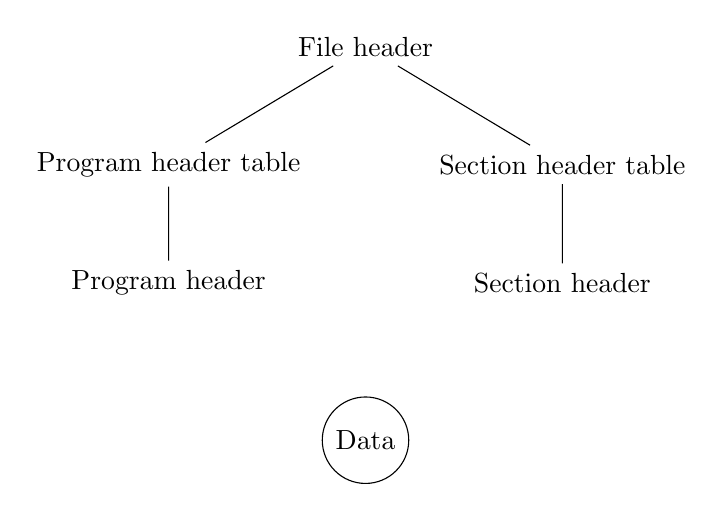
\begin{tikzpicture}[sibling distance=5cm, every node/.style={align=center}]
  \node {File header}
    child { node {Program header table}
      child { node {Program header} }
    }
    child { node {Section header table}
      child { node {Section header} }
    };

  \node [circle, draw] at (0, -5) {Data};
\end{tikzpicture}
\end{center}

\subsection{File header}

The beginning 16 bytes of the file are byte order agnostic.
The first byte must have the value $(7\text{F})_{16}$ (127) followed by
$(45)_{16}$, $(4\text{C})_{16}$, and $(46)_{16}$ (ELF in ASCII encoding).

\subsection{Program header table}

\subsection{Section header table}

This section is only used for linking(?).

  \chapter{Linking}

\section{Procedure Linkage Table (PLT)}

TODO.

  \chapter{Parallelism}

\section{Limitations}

\subsection{Amdahl's Law}

Let $N$ be the number of parallel executions.

\noindent Let $S$ be the fraction of serial runtime for a serial execution.

\noindent Let $P$ be the fraction of parallel runtime for a serial execution.

\vspace{1em}

$\text{speedup} = \frac{1}{S + \frac{P}{N}}$

\subsection{Gustafson's Law}

Let $N$ be the number of parallel executions.

\noindent Let $n$ be a measure of the problem size.

\noindent Let $S(n)$ be the fraction of serial runtime for a parallel
execution.

\noindent Let $P(n)$ be the fraction of parallel runtime for a parallel
execution.

\vspace{1em}

$\text{speedup} = S(n) + N \cdot P(n)$

  \chapter{Syntax Analysis}

\section{Lexing}

A finite state machine (FSA).

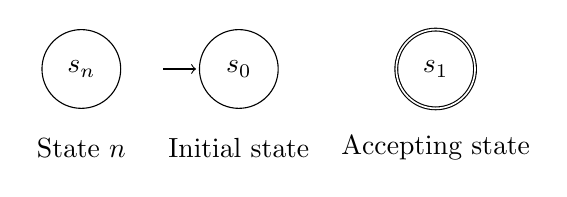
\begin{tikzpicture}[shorten >=1pt, initial text=]
  \tikzstyle{every state}=[node distance=2cm, minimum size=1cm]
  \tikzstyle{accepting}=[double]

  \node[state]                                 (sn)               {$s_n$};
  \node[state, initial]                        (s0) [right of=sn] {$s_0$};
  \node[state, accepting, node distance=2.5cm] (s1) [right of=s0] {$s_1$};
  \node[below of=sn] {State $n$};
  \node[below of=s0] {Initial state};
  \node[below of=s1] {Accepting state}; 
\end{tikzpicture}

\section{Parsing}

  \chapter{Static Analysis}

\section{Terminology}

\begin{description}
  \item[Soundness.] Never report a definite results when the opposite is true.
  \item[Precision.] Reporting a definite result as often as possible.
  \item[Conservative.] Just report ``maybe'' when in doubt.
  \item[Poset.] A partially ordered set.
  \item[Lattice.] Poset with a least upper bound (join) and greatest lower bound
                  (meet).
\end{description}

\section{Control Flow Graph (CFG)}

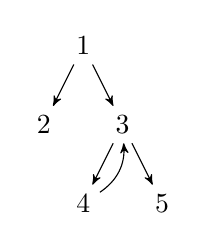
\begin{tikzpicture}[->,>=stealth']
  \node (1) {1};
  \node (2) [below of=1, xshift=-5mm] {2};
  \node (3) [right of=2] {3};
  \node (4) [below of=3, xshift=-5mm] {4};
  \node (5) [right of=4] {5};

  \path (1) edge (2)
        (1) edge (3)
        (3) edge (4)
        (4) edge [bend right] (3)
        (3) edge (5);
\end{tikzpicture}

\section{Dominator Trees}

\begin{tikzpicture}
  \node {1}
    child { node {2}
    }
    child { node {3}
      child { node {4} 
        child { node {5} }
        child { node {6} }
        child { node {7} }
      }
    };
\end{tikzpicture}

\section{Interprocedural, Finite, Distributive, Subset (IFDS)}

  \chapter{Linux Internals}

\section{Development}

\subsection{Kernel Space vs. User Space}

\subsection{Kobject}

  \chapter{Linux API}

All system calls return a word (64 bits on x86-64).

\verb+read+

\verb+write+

\verb+open+

\verb+close+

\verb+stat+

\verb+fstat+

\verb+lstat+

\verb+poll+

\verb+lseek+

\verb+mmap+

\verb+mprotect+

\verb+munmap+

\verb+brk+

\verb+rt_sigaction+

\verb+rt_sigprocmask+

\verb+rt_sigreturn+

\verb+ioctl+

\verb+pread64+

\verb+pwrite64+

\verb+readv+

\verb+writev+

\verb+access+

\verb+pipe+

\verb+select+

\verb+sched_yield+

\verb+mremap+

\verb+msync+

\verb+mincore+

\verb+madvise+

\verb+shmget+

\verb+shmat+

\verb+shmctl+

\verb+dup+

\verb+dup2+

\verb+pause+

\verb+nanosleep+

\verb+getitimer+

\verb+alarm+

\verb+setitimer+

\verb+getpid+

\verb+sendfile+

\verb+socket+

\verb+connect+

\verb+accept+

\verb+sendto+

\verb+recvfrom+

\verb+sendmsg+

\verb+recvmsg+

\verb+shutdown+

\verb+bind+

\verb+listen+

\verb+getsockname+

\verb+getpeername+

\verb+socketpair+

\verb+setsockopt+

\verb+getsockopt+

\verb+clone+

\verb+fork+

\verb+vfork+

\verb+execve+

\verb+exit+

\verb+wait4+

\verb+kill+

\verb+uname+

\verb+semget+

\verb+semop+

\verb+semctl+

\verb+shmdt+

\verb+msgget+

\verb+msgsnd+

\verb+msgrcv+

\verb+msgctl+

\verb+fcntl+

\verb+flock+

\verb+fsync+

\verb+fdatasync+

\verb+truncate+

\verb+ftruncate+

\verb+getdents+

\verb+getcwd+

\verb+chdir+

\verb+fchdir+

\verb+rename+

\verb+mkdir+

\verb+rmdir+

\verb+creat+

\verb+link+

\verb+unlink+

\verb+symlink+

\verb+readlink+

\verb+chmod+

\verb+fchmod+

\verb+chown+

\verb+fchown+

\verb+lchown+

\verb+umask+

\verb+gettimeofday+

\verb+getrlimit+

\verb+getrusage+

\verb+sysinfo+

\verb+times+

\verb+ptrace+

\verb+getuid+

\verb+syslog+

\verb+getgid+

\verb+setuid+

\verb+setgid+

\verb+geteuid+

\verb+getegid+

\verb+setpgid+

\verb+getppid+

\verb+getpgrp+

\verb+setsid+

\verb+setreuid+

\verb+setregid+

\verb+getgroups+

\verb+setgroups+

\verb+setresuid+

\verb+getresuid+

\verb+setresgid+

\verb+getresgid+

\verb+getpgid+

\verb+setfsuid+

\verb+setfsgid+

\verb+getsid+

\verb+capget+

\verb+capset+

\verb+rt_sigpending+

\verb+rt_sigtimedwait+

\verb+rt_sigqueueinfo+

\verb+rt_sigsuspend+

\verb+sigaltstack+

\verb+utime+

\verb+mknod+

\verb+uselib+

\verb+personality+

\verb+ustat+

\verb+statfs+

\verb+fstatfs+

\verb+sysfs+

\verb+getpriority+

\verb+setpriority+

\verb+sched_setparam+

\verb+sched_getparam+

\verb+sched_setscheduler+

\verb+sched_getscheduler+

\verb+sched_get_priority_max+

\verb+sched_get_priority_min+

\verb+sched_rr_get_interval+

\verb+mlock+

\verb+munlock+

\verb+mlockall+

\verb+munlockall+

\verb+vhangup+

\verb+modify_ldt+

\verb+pivot_root+

\verb+sysctl+

\verb+prctl+

\verb+arch_prctl+

\verb+adjtimex+

\verb+setrlimit+

\verb+chroot+

\verb+sync+

\verb+acct+

\verb+settimeofday+

\verb+mount+

\verb+umount2+

\verb+swapon+

\verb+swapoff+

\verb+reboot+

\verb+sethostname+

\verb+setdomainname+

\verb+iopl+

\verb+ioperm+

\verb+create_module+

\verb+init_module+

\verb+delete_module+

\verb+get_kernel_syms+

\verb+query_module+

\verb+quotactl+

\verb+nfsservctl+

\verb+getpmsg+

\verb+putpmsg+

\verb+afs_syscall+

\verb+tuxcall+

\verb+security+

\verb+gettid+

\verb+readahead+

\verb+setxattr+

\verb+lsetxattr+

\verb+fsetxattr+

\verb+getxattr+

\verb+lgetxattr+

\verb+fgetxattr+

\verb+listxattr+

\verb+llistxattr+

\verb+flistxattr+

\verb+removexattr+

\verb+lremovexattr+

\verb+fremovexattr+

\verb+tkill+

\verb+time+

\verb+futex+

\verb+sched_setaffinity+

\verb+sched_getaffinity+

\verb+set_thread_area+

\verb+io_setup+

\verb+io_destroy+

\verb+io_getevents+

\verb+io_submit+

\verb+io_cancel+

\verb+get_thread_area+

\verb+lookup_dcookie+

\verb+epoll_create+

\verb+epoll_ctl_old+

\verb+epoll_wait_old+

\verb+remap_file_pages+

\verb+getdents64+

\verb+set_tid_address+

\verb+restart_syscall+

\verb+semtimedop+

\verb+fadvise64+

\verb+timer_create+

\verb+timer_settime+

\verb+timer_gettime+

\verb+timer_getoverrun+

\verb+timer_delete+

\verb+clock_settime+

\verb+clock_gettime+

\verb+clock_getres+

\verb+clock_nanosleep+

\verb+exit_group+

\verb+epoll_wait+

\verb+epoll_ctl+

\verb+tgkill+

\verb+utimes+

\verb+vserver+

\verb+mbind+

\verb+set_mempolicy+

\verb+get_mempolicy+

\verb+mq_open+

\verb+mq_unlink+

\verb+mq_timedsend+

\verb+mq_timedreceive+

\verb+mq_notify+

\verb+mq_getsetattr+

\verb+kexec_load+

\verb+waitid+

\verb+add_key+

\verb+request_key+

\verb+keyctl+

\verb+ioprio_set+

\verb+ioprio_get+

\verb+inotify_init+

\verb+inotify_add_watch+

\verb+inotify_rm_watch+

\verb+migrate_pages+

\verb+openat+

\verb+mkdirat+

\verb+mknodat+

\verb+fchownat+

\verb+futimesat+

\verb+newfstatat+

\verb+unlinkat+

\verb+renameat+

\verb+linkat+

\verb+symlinkat+

\verb+readlinkat+

\verb+fchmodat+

\verb+faccessat+

\verb+pselect6+

\verb+ppoll+

\verb+unshare+

\verb+set_robust_list+

\verb+get_robust_list+

\verb+splice+

\verb+tee+

\verb+sync_file_range+

\verb+vmsplice+

\verb+move_pages+

\verb+utimensat+

\verb+epoll_pwait+

\verb+signalfd+

\verb+timerfd_create+

\verb+eventfd+

\verb+fallocate+

\verb+timerfd_settime+

\verb+timerfd_gettime+

\verb+accept4+

\verb+signalfd4+

\verb+eventfd2+

\verb+epoll_create1+

\verb+dup3+

\verb+pipe2+

\verb+inotify_init1+

\verb+preadv+

\verb+pwritev+

\verb+rt_tgsigqueueinfo+

\verb+perf_event_open+

\verb+recvmmsg+

\verb+fanotify_init+

\verb+fanotify_mark+

\verb+prlimit64+

\verb+name_to_handle_at+

\verb+open_by_handle_at+

\verb+clock_adjtime+

\verb+syncfs+

\verb+sendmmsg+

\verb+setns+

\verb+getcpu+

\verb+process_vm_readv+

\verb+process_vm_writev+

\verb+kcmp+

\verb+finit_module+

\verb+sched_setattr+

\verb+sched_getattr+

\verb+renameat2+

\verb+seccomp+

\verb+getrandom+

\verb+memfd_create+

\verb+kexec_file_load+

\verb+bpf+

\verb+execveat+

  \chapter{Wayland}

Wayland is a protocol for graphics and input intended for applications.

\textit{Background knowledge: UNIX domain stream socket.}

\newpage

\section{Objects}

Each object has a set of requests and events.

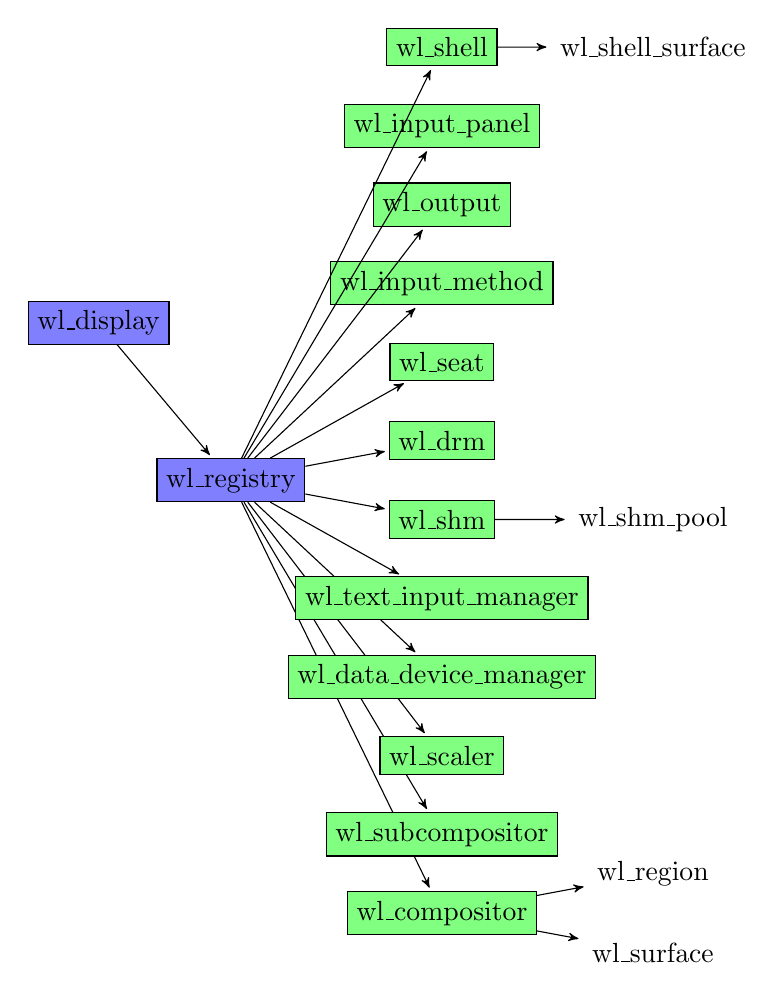
\begin{tikzpicture}[->,>=stealth',shorten >=0.5mm,grow=right,
                    level distance=2.68cm,sibling distance=1cm]
  \tikzstyle{core} = [draw, rectangle, fill=blue!50]
  \tikzstyle{global} = [draw, rectangle, fill=green!50]
  \node [core] {wl\_display}
    child {
      node [core, xshift=-1cm, yshift=-2cm] {wl\_registry}
        child {
          node [global] {wl\_compositor}
            child {
              node {wl\_surface}
            }
            child {
              node {wl\_region}
            }
        }
        child {
          node [global] {wl\_subcompositor}
        }
        child {
          node [global] {wl\_scaler}
        }
        child {
          node [global] {wl\_data\_device\_manager}
        }
        child {
          node [global] {wl\_text\_input\_manager}
        }
        child {
          node [global] {wl\_shm}
            child {
              node {wl\_shm\_pool}
            }
        }
        child {
          node [global] {wl\_drm}
        }
        child {
          node [global] {wl\_seat}
        }
        child {
          node [global] {wl\_input\_method}
        }
        child {
          node [global] {wl\_output}
        }
        child {
          node [global] {wl\_input\_panel}
        }
        child {
          node [global] {wl\_shell}
            child {
              node {wl\_shell\_surface}
            }
        }
    }
  ;
\end{tikzpicture}

\newpage
\subsection{wl\_output}

\subsubsection{Events}

\paragraph{geometry}

\begin{enumerate}
  \item x
  \item y
  \item physical\_width (unit: mm)
  \item physical\_height (unit: mm)
  \item subpixel
  \item make
  \item model
  \item transform
\end{enumerate}


  \chapter{Vulkan}

\section{Overview}

\section{$n$-body Problem}

Let $M_{\odot}$ be the solar mass.

$M_{\odot} = \frac{4\pi^2 \times (1 \text{ AU})^3}{G \times (1 \text{ yr})^2}$

\noindent Units of $G$ are:

$\text{N} \text{ m}^2 \text{ kg}^{-2}
  = \text{m}^3 \text{ kg}^{-1} \text{ s}^{-2}$

\paragraph{Energy.}

Given by the equation:  

$\sum\limits_{i=1}^n \sum\limits_{j=1, j \neq i}^n \frac{m_i m_j}{r_{ij}}$

  \chapter{Audio}

On Linux, there's currently ALSA, and PulseAudio.

  \chapter{Cryptography}

\section{Information Theory}

\subsection{Hamming Distance}

A measure of how many characters are different in two strings of equal length.

Example: Consider the two ASCII encoded strings ``this is a test'' and ``wokka
wokka!!!''. Both have the same length of 14 characters. If each character is
represented as 8 bits we have to many 112 comparsions ($14 \times 8$).

\texttt{t} is $116 = (74)_{16} = (01110100)_{2}$

\texttt{w} is $119 = (77)_{16} = (01110111)_{2}$

This hamming distance between these two characters is 2.

\texttt{h} is $104 = (68)_{16} = (01101000)_{2}$

\texttt{o} is $111 = (6\text{F})_{16} = (01101111)_{2}$

This hamming distance between these two characters is 3, running total of 5.

\texttt{i} is $105 = (69)_{16} = (01101001)_{2}$

\texttt{k} is $107 = (6\text{B})_{16} = (01101011)_{2}$

This hamming distance between these two characters is 1, running total of 6.

And so on, the hamming distance of these two strings is 37.

\section{Block Ciphers}

\subsection{Modes of Operation}

\subsubsection{Electronic Codebook (ECB)}

\subsubsection{Cipher Block Chaining (CBC)}

\subsubsection{Counter (CTR)}

  \chapter{History}

\begin{description}
  \item[John Wilder Tukey] Coined the term \textit{bit}.
  \item[George Boole] Work in logic, root of \textit{boolean}.
  \item[Homer Dudley] First electronic voice synthesizer, and first encrypted
                      voice transmissions.
\end{description}


\end{document}
